\documentclass[]{report}
\usepackage{graphicx}

% Title Page
\title{A Report into the Relationship between Tax, GDP and Regulatory Environment}
\author{Your name goes here}

\begin{document}
	\maketitle
	
	\begin{abstract}
		A Report compiled for the Alliance of Wealthy People who Dislike Tax, investigating the relationship between rates of taxation (measured as a percentage of GDP), regulatory environment (measured through the World Bank's Ease of Doing Business), and GDP per capita (measured in current US dollars). Data are for European and Central Asian countries for the year 2019.
	\end{abstract}
	
	\section{Findings}
	A multivariate regression of the variables resulted in the following findings:
	
	% Table created by stargazer
	\begin{table}[!htbp] \centering 
		\caption{Regression Results: GDP per capita vs Tax and Regulation} 
		\label{tab:regression} 
		\begin{tabular}{@{\extracolsep{5pt}}lc} 
			\\[-1.8ex]\hline 
			\hline \\[-1.8ex] 
			& \multicolumn{1}{c}{\textit{Dependent variable:}} \\ 
			\cline{2-2} 
			% FIXED: Added backslashes before $ and %
			\\[-1.8ex] & GDP per capita (current US\$) \\ 
			\hline \\[-1.8ex] 
			% FIXED: Added backslash before %
			Tax revenue (\% of GDP) & 1,458.24$^{*}$ \\ 
			& (738.97) \\ 
			Ease of doing business rank & $-$222.97 \\ 
			& (162.66) \\ 
			Constant & 9,256.39 \\ 
			& (17,201.77) \\ 
			\hline \\[-1.8ex] 
			Observations & 46 \\ 
			R$^{2}$ & 0.13 \\ 
			Adjusted R$^{2}$ & 0.09 \\ 
			\hline 
			\hline \\[-1.8ex] 
			\textit{Note:}  & \multicolumn{1}{r}{$^{*}$p$<$0.1; $^{**}$p$<$0.05; $^{***}$p$<$0.01} \\ 
		\end{tabular} 
	\end{table} 
	
	The relationship can be visualised in a scatter plot.
	
	\begin{figure}[h]
		\centering
		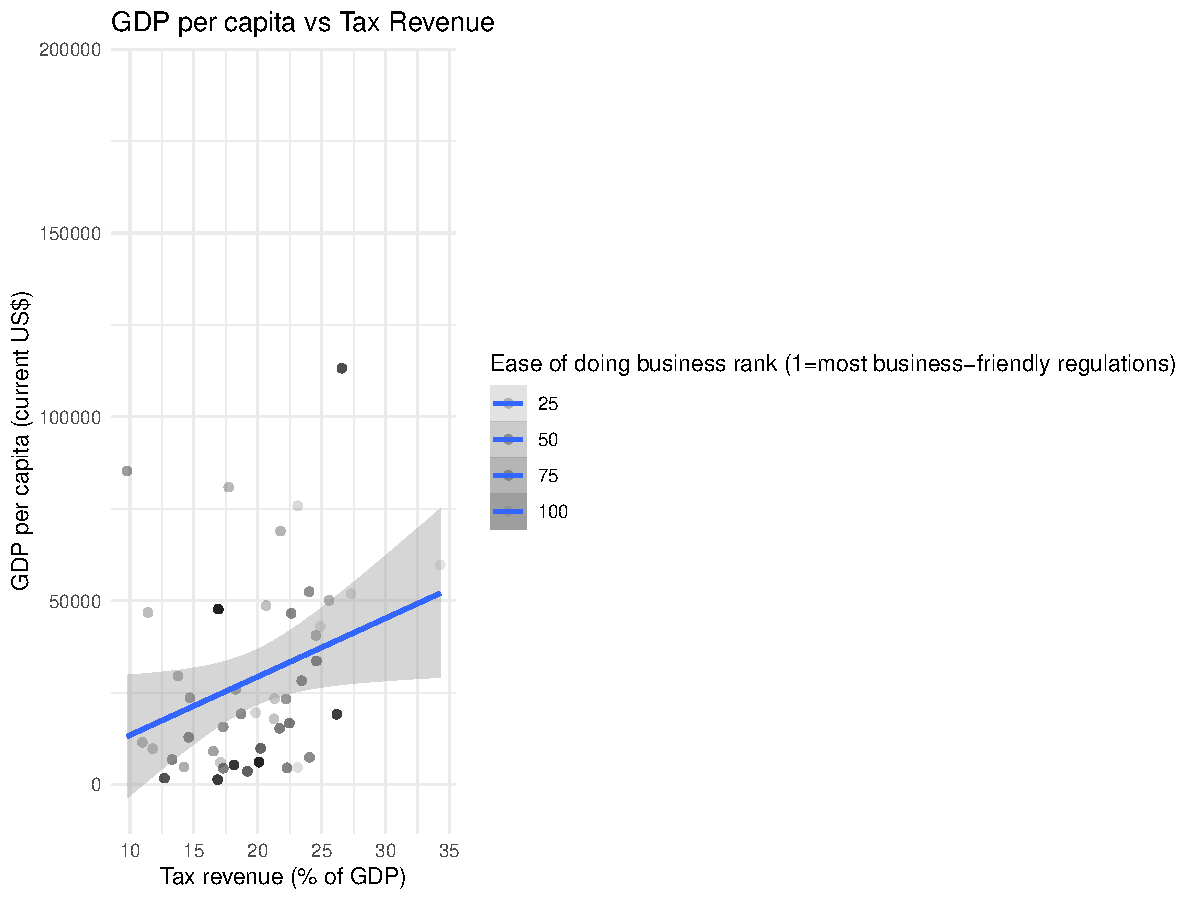
\includegraphics[page=1, width=0.8\textwidth]{gdp_tax_plot.pdf}
		\caption{Scatter plot of GDP vs Tax Revenue}
		\label{fig:gdptaxplot}
	\end{figure}

	
\end{document}\\
         
